\documentclass[11pt,letterpaper]{article}
\usepackage[lmargin=1in,rmargin=1in,tmargin=1in,bmargin=1in]{geometry}
\usepackage{../style/homework}
\usepackage{../style/commands}
\setbool{quotetype}{true} % True: Side; False: Under
\setbool{hideans}{false} % Student: True; Instructor: False

% -------------------
% Content
% -------------------
\begin{document}

\homework{1: Due 02/08}{Windows are the eyes to the house.}{Andy Dwyer, Parks \& Recreation}

% Problem 1
\problem{10} Give the definition of a real number. Also, give at least five original examples of a real number. \pspace

{\itshape A real number is `any' number which is expressible as a decimal, e.g.
	\[
	\begin{aligned}
	0&= 0.0 \\[0.3cm]
	1&= 1.0 \\[0.3cm]
	-5&= -5.0 \\[0.3cm]
	\dfrac{1}{2}&= 0.5 \\[0.3cm]
	-\dfrac{1}{10}&= -0.1 \\[0.3cm]
	0.119589&04771 \\[0.3cm]
	\sqrt{2}= 1.4142135&62373095\ldots \\[0.3cm]
	\pi= 3.14159265&3589793\ldots \\[0.3cm]
	e= 2.71828182&8495045\ldots \\[0.3cm]
	\gamma= 0.577215&664901532\ldots
	\end{aligned}
	\]
}



\newpage



% Problem 2
\problem{10} Give the definition of a rational number. Also, give at least five original examples of a rational number. \pspace

{\itshape A rational number is a real number of the form $\frac{a}{b}$, where $a$ and $b$ are integers and $b \neq 0$, e.g.
	\[
	\begin{aligned}
	0&= \dfrac{0}{1} \\[0.3cm]
	2&= \dfrac{2}{1} \\[0.3cm]
	-5&= -\dfrac{5}{1} \\[0.3cm]
	\phantom{=}& \dfrac{1}{2} \\[0.3cm]
	-\phantom{=}&\dfrac{5}{7} \\[0.3cm]
	\phantom{.}&\dfrac{20}{100} 
	\end{aligned}
	\]
}



\newpage



% Problem 3
\problem{10} Find the prime factorizations of the following integers:
	\begin{enumerate}[(a)]
	\item $54$
	\item $97$
	\item $168$
	\item $184$
	\end{enumerate} \pspace

\sol
\begin{enumerate}[(a)]
\item $54= 2 \cdot 3^3$
	\[
	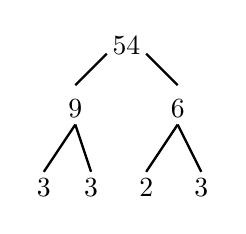
\begin{tikzpicture}
	\node at (-0.15,0) {$54$};
	\draw[line width=0.03cm] (-0.4,-0.1) -- (-0.8,-0.5);
	\node at (-0.8,-0.8) {$9$};
	\draw[line width=0.03cm]  (0.1,-0.1) -- (0.5,-0.5);
	\node at (0.5,-0.8) {$6$};
		
	\draw[line width=0.03cm] (-0.8,-1) -- (-1.2,-1.6);
	\node at (-1.2,-1.8) {$3$};
	\draw[line width=0.03cm] (-0.8,-1) -- (-0.6,-1.6);
	\node at (-0.6,-1.8) {$3$};
	
	\draw[line width=0.03cm] (0.5,-1) -- (0.1,-1.6);
	\node at (0.1,-1.8) {$2$};
	\draw[line width=0.03cm] (0.5,-1) -- (0.8,-1.6);
	\node at (0.8,-1.8) {$3$};
	\end{tikzpicture}
	\] \pspace
	
\item $97= 97$ (Already prime) \pspace

\item $168= 2^3 \cdot 3 \cdot 7$
	\[
	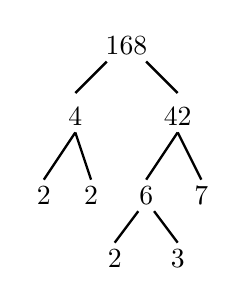
\begin{tikzpicture}
	\node at (-0.15,0.1) {$168$};
	\draw[line width=0.03cm] (-0.4,-0.1) -- (-0.8,-0.5);
	\node at (-0.8,-0.8) {$4$};
	\draw[line width=0.03cm]  (0.1,-0.1) -- (0.5,-0.5);
	\node at (0.5,-0.8) {$42$};
		
	\draw[line width=0.03cm] (-0.8,-1) -- (-1.2,-1.6);
	\node at (-1.2,-1.8) {$2$};
	\draw[line width=0.03cm] (-0.8,-1) -- (-0.6,-1.6);
	\node at (-0.6,-1.8) {$2$};
	
	\draw[line width=0.03cm] (0.5,-1) -- (0.1,-1.6);
	\node at (0.1,-1.8) {$6$};
	\draw[line width=0.03cm] (0.5,-1) -- (0.8,-1.6);
	\node at (0.8,-1.8) {$7$};
	
	\draw[line width=0.03cm] (0,-2.0) -- (-0.3,-2.4);
	\node at (-0.3,-2.6) {$2$};
	\draw[line width=0.03cm] (0.2,-2.0) -- (0.5,-2.4);
	\node at (0.5,-2.6) {$3$};
	\end{tikzpicture}
	\] \pspace

\item $184= 2^3 \cdot 23$
	\[
	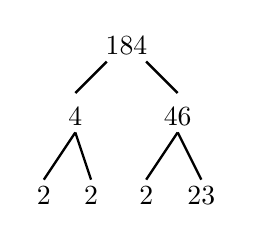
\begin{tikzpicture}
	\node at (-0.15,0.1) {$184$};
	\draw[line width=0.03cm] (-0.4,-0.1) -- (-0.8,-0.5);
	\node at (-0.8,-0.8) {$4$};
	\draw[line width=0.03cm]  (0.1,-0.1) -- (0.5,-0.5);
	\node at (0.5,-0.8) {$46$};
		
	\draw[line width=0.03cm] (-0.8,-1) -- (-1.2,-1.6);
	\node at (-1.2,-1.8) {$2$};
	\draw[line width=0.03cm] (-0.8,-1) -- (-0.6,-1.6);
	\node at (-0.6,-1.8) {$2$};
	
	\draw[line width=0.03cm] (0.5,-1) -- (0.1,-1.6);
	\node at (0.1,-1.8) {$2$};
	\draw[line width=0.03cm] (0.5,-1) -- (0.8,-1.6);
	\node at (0.8,-1.8) {$23$};
	\end{tikzpicture}
	\] 
\end{enumerate}



\newpage



% Problem 4
\problem{10} Without using a calculator, answer the following:
	\begin{enumerate}[(a)]
	\item Does 2 divide 2346? Explain.
	\item Does 3 divide 596012? Explain.
	\item Does 4 divide 990140? Explain.
	\item Does 5 divide 1431? Explain.
	\item Does 9 divide 70155? Explain. 
	\end{enumerate} \pspace

\sol
\begin{enumerate}[(a)]
\item 
\item 
\item 
\item 
\item 
\end{enumerate}



\newpage



% Problem 5
\problem{10} Using the `square root method,' show that 157 is prime. 



\newpage



% Problem 6
\problem{10} By listing out all the divisors of the given numbers, compute the following:
	\begin{enumerate}[(a)]
	\item $\gcd(12, 15)$
	\item $\gcd(20, 22)$
	\item $\gcd(36, 60)$
	\item $\gcd(20, 100)$
	\end{enumerate}



\newpage



% Problem 7
\problem{10} By listing out sufficiently many multiples of the given integers, compute the following:
	\begin{enumerate}[(a)]
	\item $\lcm(24, 36)$
	\item $\lcm(12, 15)$
	\item $\lcm(12, 18)$
	\item $\lcm(36, 48)$
	\end{enumerate}



\newpage



% Problem 8
\problem{10} By finding prime factorizations, compute the following:
	\begin{enumerate}[(a)]
	\item $\gcd(12, 15)$
	\item $\gcd(20, 22)$
	\item $\gcd(36, 60)$
	\item $\gcd(20, 100)$
	\end{enumerate}



\newpage



% Problem 9
\problem{10} By finding prime factorizations, compute the following:
	\begin{enumerate}[(a)]
	\item $\lcm(24, 36)$
	\item $\lcm(12, 15)$
	\item $\lcm(12, 18)$
	\item $\lcm(36, 48)$
	\end{enumerate}



\newpage



% Problem 10
\problem{10} Compute the following:
	\begin{enumerate}[(a)]
	\item $\gcd(2^3 \cdot 3^1 \cdot 5^3 \cdot 11^5, 2^2 \cdot 3^3 \cdot 5 \cdot 7)$
	\item $\lcm(2^3 \cdot 3^1 \cdot 5^3 \cdot 11^5, 2^2 \cdot 3^3 \cdot 5 \cdot 7)$
	\item $\gcd(2^{10} \cdot 5^5 \cdot 13, 3^5 \cdot 5^1 \cdot 11^2)$
	\item $\lcm(2^{10} \cdot 5^5 \cdot 13, 3^5 \cdot 5^1 \cdot 11^2)$
	\end{enumerate}


\end{document}